\documentclass{article}
\usepackage{listings}
\usepackage{amsmath}
\usepackage{fullpage}
\usepackage{tabularx}
\usepackage{graphicx}
\usepackage{cite}
\usepackage{hyperref}
\begin{document}
\lstset{language=python, tabsize=4}
\title{Graph mining: deep learning approaches}
\author{Yuchen Hou}
\maketitle

\begin{abstract}
	I summarize recent deep learning approaches in 2 graph mining tasks: node prediction and link prediction. The key in all these approaches is node embedding(the process of projecting every node in the graph into a point in a node space, i.e. embedding nodes in node space). The result of this process is that every node is represented by a point in the node space, where the coordinates of the point are expected to contain most information about the node related to the prediction task. This process is critical because neural nets can only handle numbers directly, which means everything needs to be converted to numbers before it can be processed by a neural net. Other aspects in these approaches are task specific and I will address them in corresponding sections.
\end{abstract}

\section{Introduction}

The idea of node embedding in graph mining can be traced back to the idea of word embedding in natural language processing, an early and famous domain where entities are conceptual or categorical instead of numerical, and relations between entities are important. This is very different from other domains including image recognition and speech recognition. Graph mining is more complex compared to the domains mentioned above, as graphs are more flexible and have all the above characteristics. Table \ref{tab:domains} provides a summary of various types of entities, their representations and intern entity relations in different domains.

\begin{table}
	\centering
	\begin{tabularx}{\textwidth}{ |c|c|X|X| }
		\hline domain & entity & representation & relations to other entities \\ 
		\hline image recognition & image & 2D pixel array & NA \\ 
		\hline speech recognition & utterance & 2D spectrogram array & NA \\ 
		\hline natural language processing & word & word vector(1D array) & relations to other words \\ 
		\hline graph mining & movie & node vector(1D array) & produced by producer, directed by director, etc \\ 
		\hline graph mining & user & node vector(1D array) & rate movies, message other users, etc \\ 
		\hline graph mining & article & node vector(1D array) & address topics, cite other articles, etc \\
		\hline
	\end{tabularx}
	\caption{A summary of various types of entities, their representations and inter-entity relations in different domains: images and utterances can be directly represented by 2D numerical arrays, but have no strong relations to other images or utterances; words and various types of nodes in graphs can also be represented by 1D numerical arrays, but have strong relations to other words and nodes.}
	\label{tab:domains}
\end{table}

In Table \ref{tab:domains}, the entities listed in the lower rows have increasing representation complexities. Pixel and spectrogram arrays for images and utterances can be measured by physical instruments from the entities themselves. Word vectors are more difficult to get because no instrument can measure words and a word vector can only be learned from the relations between the word to other words. Nodes in graphs are the most difficult to handle because of they can have many measurable attributes and also many types of relations to other entities. For example, a user has attributes like age, weight, salary, DNA sequence, has relations with other entities like rating songs, writing articles, messaging other users. Every one of these attributes and relations provides useful information about what kind of person the user is and potentially useful in a prediction task like whether this user would be interested in a specific song or article. It's not straightforward to put all the information related to nodes into a highly informative numerical vectors, but if it can be done, neural nets will be able to tackle challenging prediction tasks using these numerical vectors.

Figure \ref{fig:Airy-pattern} shows how an image is represented by a 2D pixel intensity array in image recognition. Most of us are very familiar with this representation that we often don't realize the pixel array is only one of the representations of an image.

\begin{figure}
	\centering
	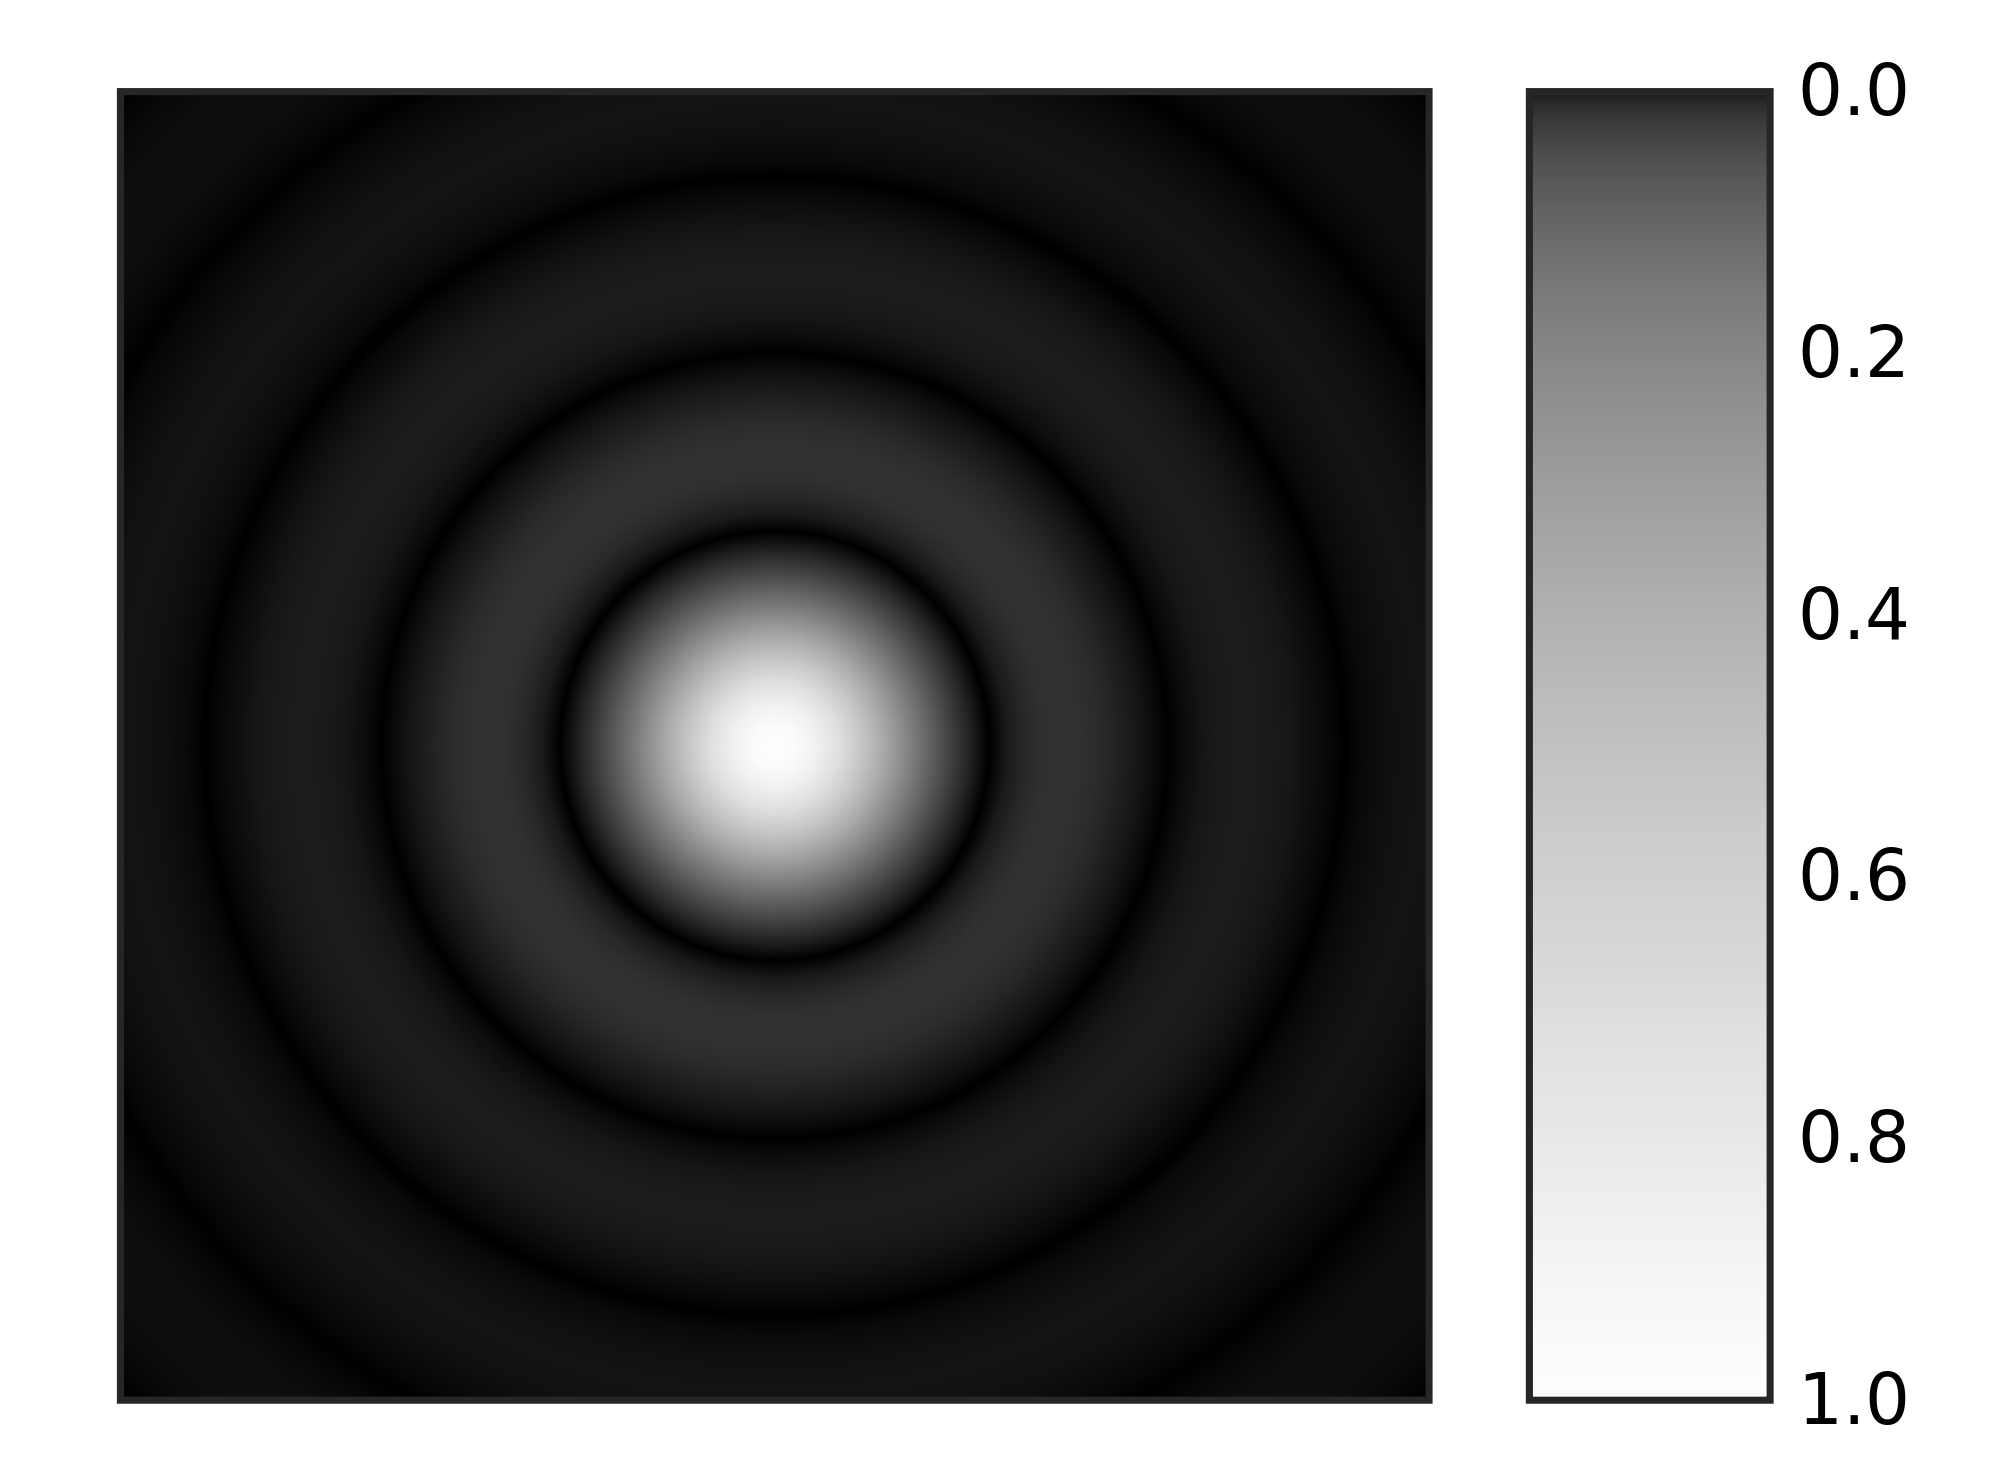
\includegraphics[width=0.5\linewidth]{Airy-pattern}
	\caption{The 2D pixel array of an image of  \href{https://commons.wikimedia.org/wiki/File:Airy-pattern.svg}{the airy pattern} (John Doe / Wikimedia Commons / Public Domain): the horizontal and vertical axes represent the width and the height; the value at a specific (width, height) location is the pixel intensity.}
	\label{fig:Airy-pattern}
\end{figure}

Figure \ref{fig:Spectrogram-19thC} shows how an utterance is represented by a 2D spectrogram array in speech recognition. Notice that this is very similar to the case of images, except the 2 axes have different meanings now - time and frequency. However, this subtle difference does lead to very different techniques in deep learning applications in the 2 domains.

\begin{figure}
	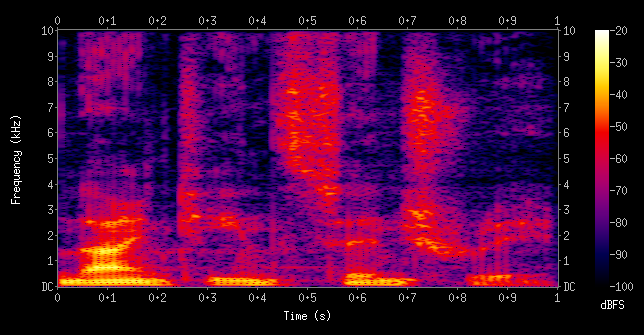
\includegraphics[width=\linewidth]{Spectrogram-19thC}
	\caption{The 2D spectrogram array of \href{https://commons.wikimedia.org/wiki/File:Spectrogram-19thC.png}{a male voice saying "nineteenth century"}(Aquegg / Wikimedia Commons / Public Domain): the value at a specific (time, frequency) location is the sound intensity measured in unit dBFS(decibel relative to full scale).}
	\label{fig:Spectrogram-19thC}
\end{figure}

Table

\begin{table}
	\centering
	\begin{tabularx}{\textwidth}{ |c|X| }
	\end{tabularx}
	\caption{}
\end{table}

In the next few sections I present a few different deep learning approaches in node embedding and various graph prediction tasks:
\begin{itemize}
	\item Section 2: SkipGram approach\cite{perozzi2014deepwalk}
\end{itemize}


\section{Node prediction: DeepWalk}


\section{Node prediction:others}

\section{Link prediction}

\subsection{Graphs with rich node attributes and link attributes}
In some prediction tasks, graphs need to incorporate rich attributes in nodes and links to take advantage of large amount of available information. This becomes significant in scenarios where a service provider allows a wide range of activities from the users and record these activities. The popular Amazon e-commerce service is a good example, which records these activities as available information:
\begin{enumerate}
	\item buyers can buy, rate, write reviews, post questions and answers for products, and rate, write reviews for sellers, 
	\item manufactures produce, write descriptions for products
	\item sellers sell, write advertisements for products
\end{enumerate}
Beside these activities, buyers, manufactures and sellers have very limited information about themselves in their profile, while products have richer information like price, category, specs. Having all this comprehensive information in hand, it is of great interest to the service provider to.

\bibliographystyle{acm}
\bibliography{references}

\end{document}